\documentclass[UTF8]{ctexart}
\usepackage{geometry}
\usepackage{pdfpages}
\usepackage{titlesec}
\usepackage{graphicx}
\usepackage{grffile}
\usepackage{booktabs}
\geometry{a4paper, margin=1in}

% 一级标题：二号黑体，居中
\titleformat{\section}{\centering\heiti\zihao{-2}}{\thesection}{1em}{}
% 二级标题：三号黑体，靠左
\titleformat{\subsection}{\heiti\zihao{-3}}{\thesubsection}{1em}{}
% 三级标题：四号黑体，靠左（按需使用）
\titleformat{\subsubsection}{\heiti\zihao{-4}}{\thesubsubsection}{1em}{}

% 正文：五号宋体
\AtBeginDocument{\songti\zihao{-5}}

\title{Software Design}
\author{}
\date{\today}

\renewcommand{\contentsname}{目录}
\setcounter{secnumdepth}{0}

\begin{document}

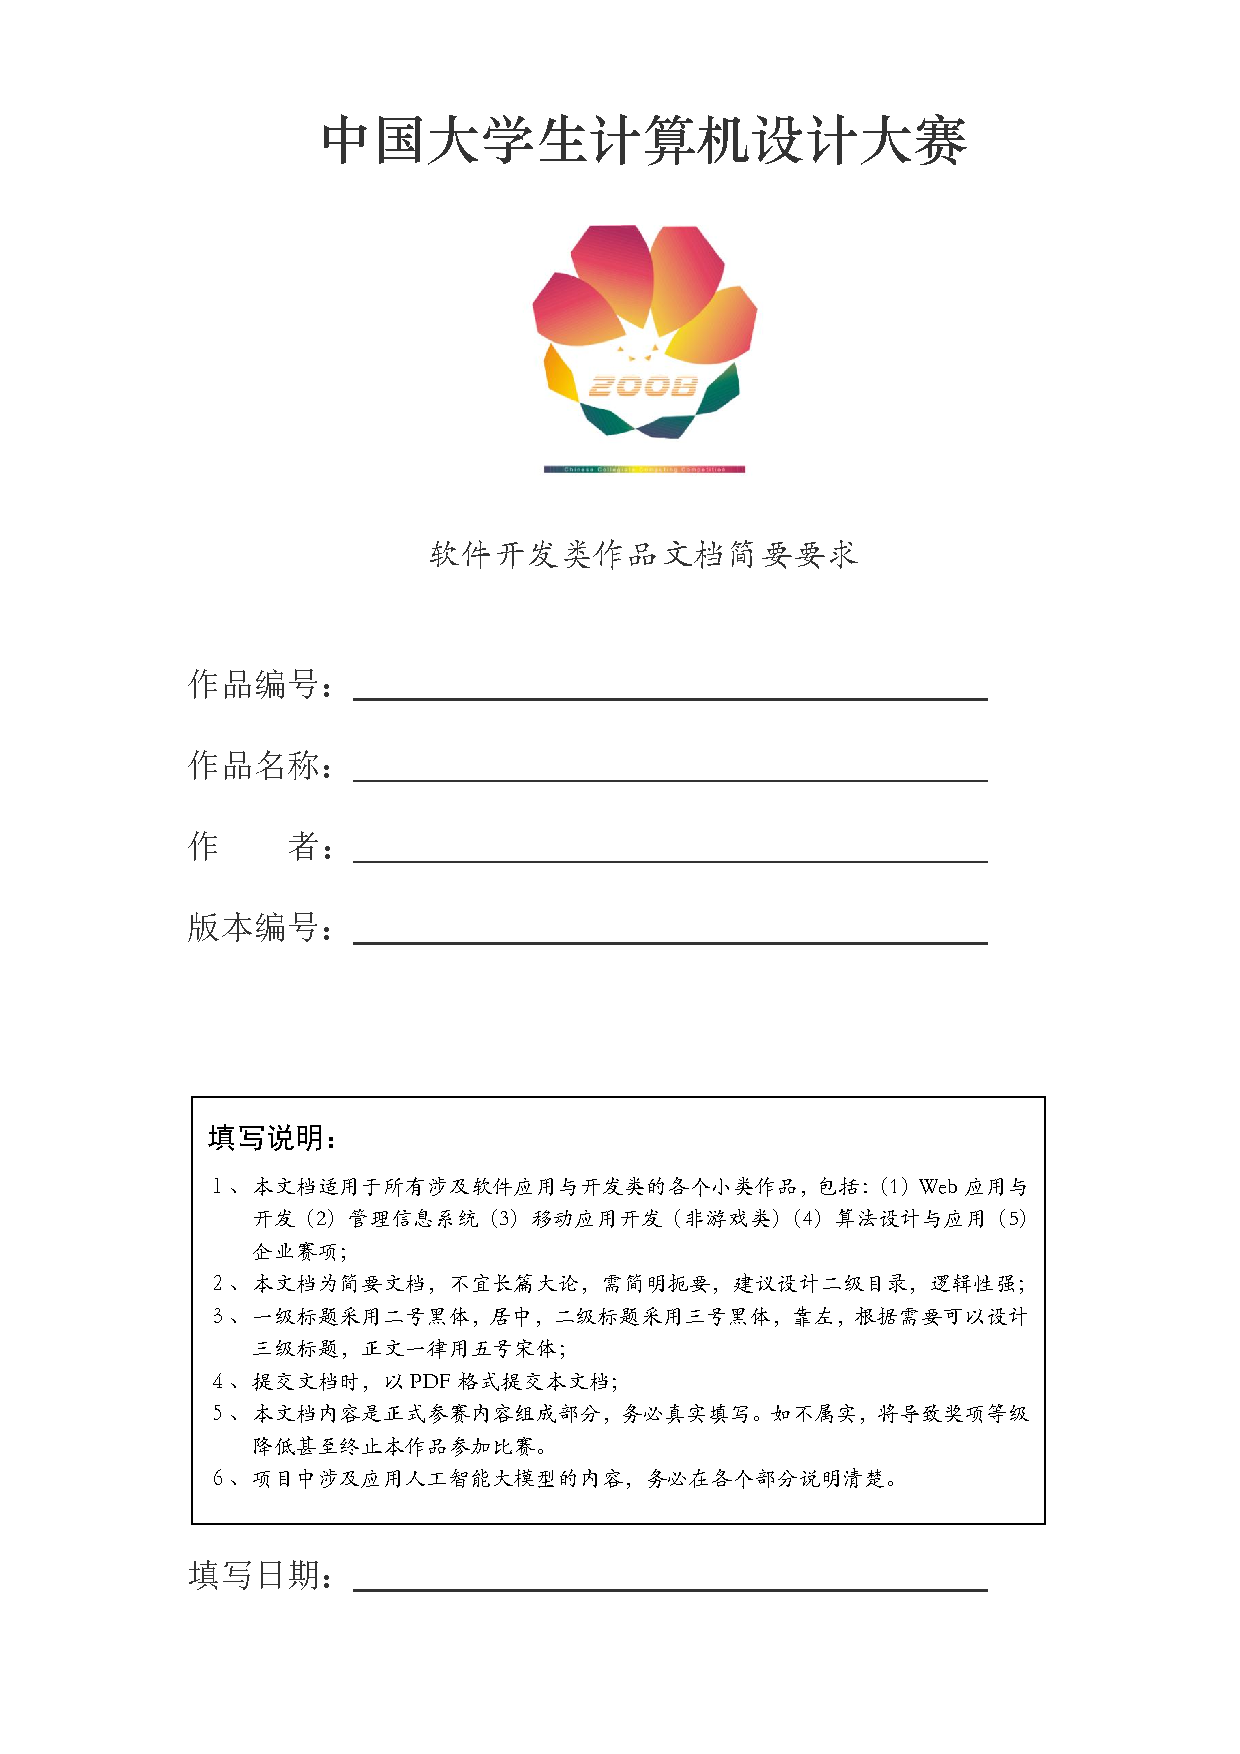
\includepdf[pages=1]{template.pdf}

\maketitle

\tableofcontents
\newpage

\section{第一章\quad 需求分析}
随着跨设备远程协助需求持续增长，用户对远程控制系统提出了更明确的期望，即在手机、平板与桌面端之间实现低门槛接入、低时延交互和可审计的会话过程。结合远程桌面市场的持续扩张趋势，以及国内物联网与智能终端场景的快速普及，本系统定位为面向教育演示、家庭设备维护和中小团队技术支持的轻量化远程桌面控制工具，并将“连接稳定性、操作流畅度、数据安全性”作为核心体验目标。为满足差异化体验需求，系统采用“原生HarmonyOS端+Flutter端+桌面端”的三端协同方案，针对各终端独有的操作逻辑进行特化设计：HarmonyOS端侧重分布式场景下的轻量连接与触控效率，Flutter端侧重跨平台界面一致性与快速迭代能力，桌面端侧重键鼠精细控制、窗口化管理和长时会话稳定性，从而在不同设备上提供一致且高效的使用体验。结合图示的目标用户与应用场景，系统主要服务于远程办公人员、IT技术支持人员、远程教育工作者和系统管理员四类人群，并围绕其业务需求提供跨网络设备连接、实时屏幕采集与显示、远程输入控制、会话管理、基础文件/信息交互及加密传输等能力，以支撑远程办公、技术支持、在线教学和服务器管理等典型应用场景。

\begin{figure}[h]
\centering
\includegraphics[width=0.88\textwidth]{../reference/picture/目标用户与应用场景图.png}
\caption{目标用户与应用场景图}
\end{figure}

主要性能需求如下：在常见宽带网络条件下，优先保障连接成功率与会话连续性；控制操作应具备可感知的低时延；系统在长时会话下应保持稳定，不因短时网络抖动导致频繁断连；关键控制行为可追踪，满足基本运维审计需求。

\begin{table}[h]
\centering
\caption{竞品技术对比分析表}
\small
\setlength{\tabcolsep}{3pt}
\renewcommand{\arraystretch}{1.2}
\begin{tabular}{p{2.4cm}p{3.9cm}p{3.9cm}p{3.9cm}}
\toprule
技术对比维度 & 本作品（自研远控系统） & TeamViewer（国际通用远控） & 向日葵（国内通用远控） \\
\midrule
目标场景 & 远程办公/技术支持/远程教学/服务器运维；三端协同（HarmonyOS+Java+服务端） & 企业级跨区域远程支持，覆盖多平台终端 & 个人与企业通用远控，偏国内网络与运维场景 \\
连接协议 & TCP长连接+自定义二进制协议，Ping/Pong心跳；文件与剪贴板走HTTP分流 & 自研RDP衍生协议，TLS 1.3，跨公网延迟80-150ms & RDP/VNC二次开发，公网延迟60-120ms \\
连接体验 & 配置与状态统一管理；支持自动重连、心跳保活、连接状态回调 & 功能完整但配置较重，需账号绑定 & 上手较快，支持扫码配对与设备分组 \\
安全与合规 & 设备凭证校验、协议边界检查、校验和与日志；预留TLS/审计扩展 & 支持MFA与分级管控，符合GDPR/ISO 27001 & 本地化合规较强，支持日志留存与敏感操作预警 \\
成本与部署 & 开源技术栈（Java+Netty+ArkTS）；支持本地构建与私有化部署 & 商业授权成本高，私有化需额外授权 & 商业版分层明显，企业版支持私有化 \\
性能指标 & 分块增量传输、缓存合并、RLE+ZSTD、缓冲区复用；maxFps默认30（可配） & 支持4K，30fps，CPU 10-15\%（单会话） & 支持1080P，20-25fps，CPU 8-12\%（单会话） \\
差异化技术定位 & 协议兼容+三端特化；主线程PixelMap渲染，依赖注入便于扩展 & 平台化与生态能力强，适合大规模集群管控 & 本地网络优化与易用性强，国内服务响应较快 \\
\bottomrule
\end{tabular}
\end{table}

\section{第二章\quad 概要设计}
本章从系统分层结构、端侧组件协同关系以及端到端数据流三个视角说明总体方案，突出模块解耦、链路可观测与跨端协同能力。

\begin{figure}[h]
\centering
\includegraphics[width=0.92\textwidth]{../reference/picture/HarmonyOS组件架构图.png}
\caption{HarmonyOS组件架构图}
\end{figure}

\begin{figure}[h]
\centering
\includegraphics[width=0.92\textwidth]{../reference/picture/Java端组件关系图.png}
\caption{Java端组件关系图}
\end{figure}

\begin{figure}[h]
\centering
\includegraphics[width=0.92\textwidth]{../reference/picture/端到端数据流.png}
\caption{端到端数据流}
\end{figure}

\section{第三章\quad 详细设计}
本章围绕客户端交互入口、图像采集与编码链路、网络异步处理机制以及压缩策略展开详细设计，重点说明关键模块如何在保证画面质量的同时降低带宽占用并提升链路稳定性。

\begin{figure}[h]
\centering
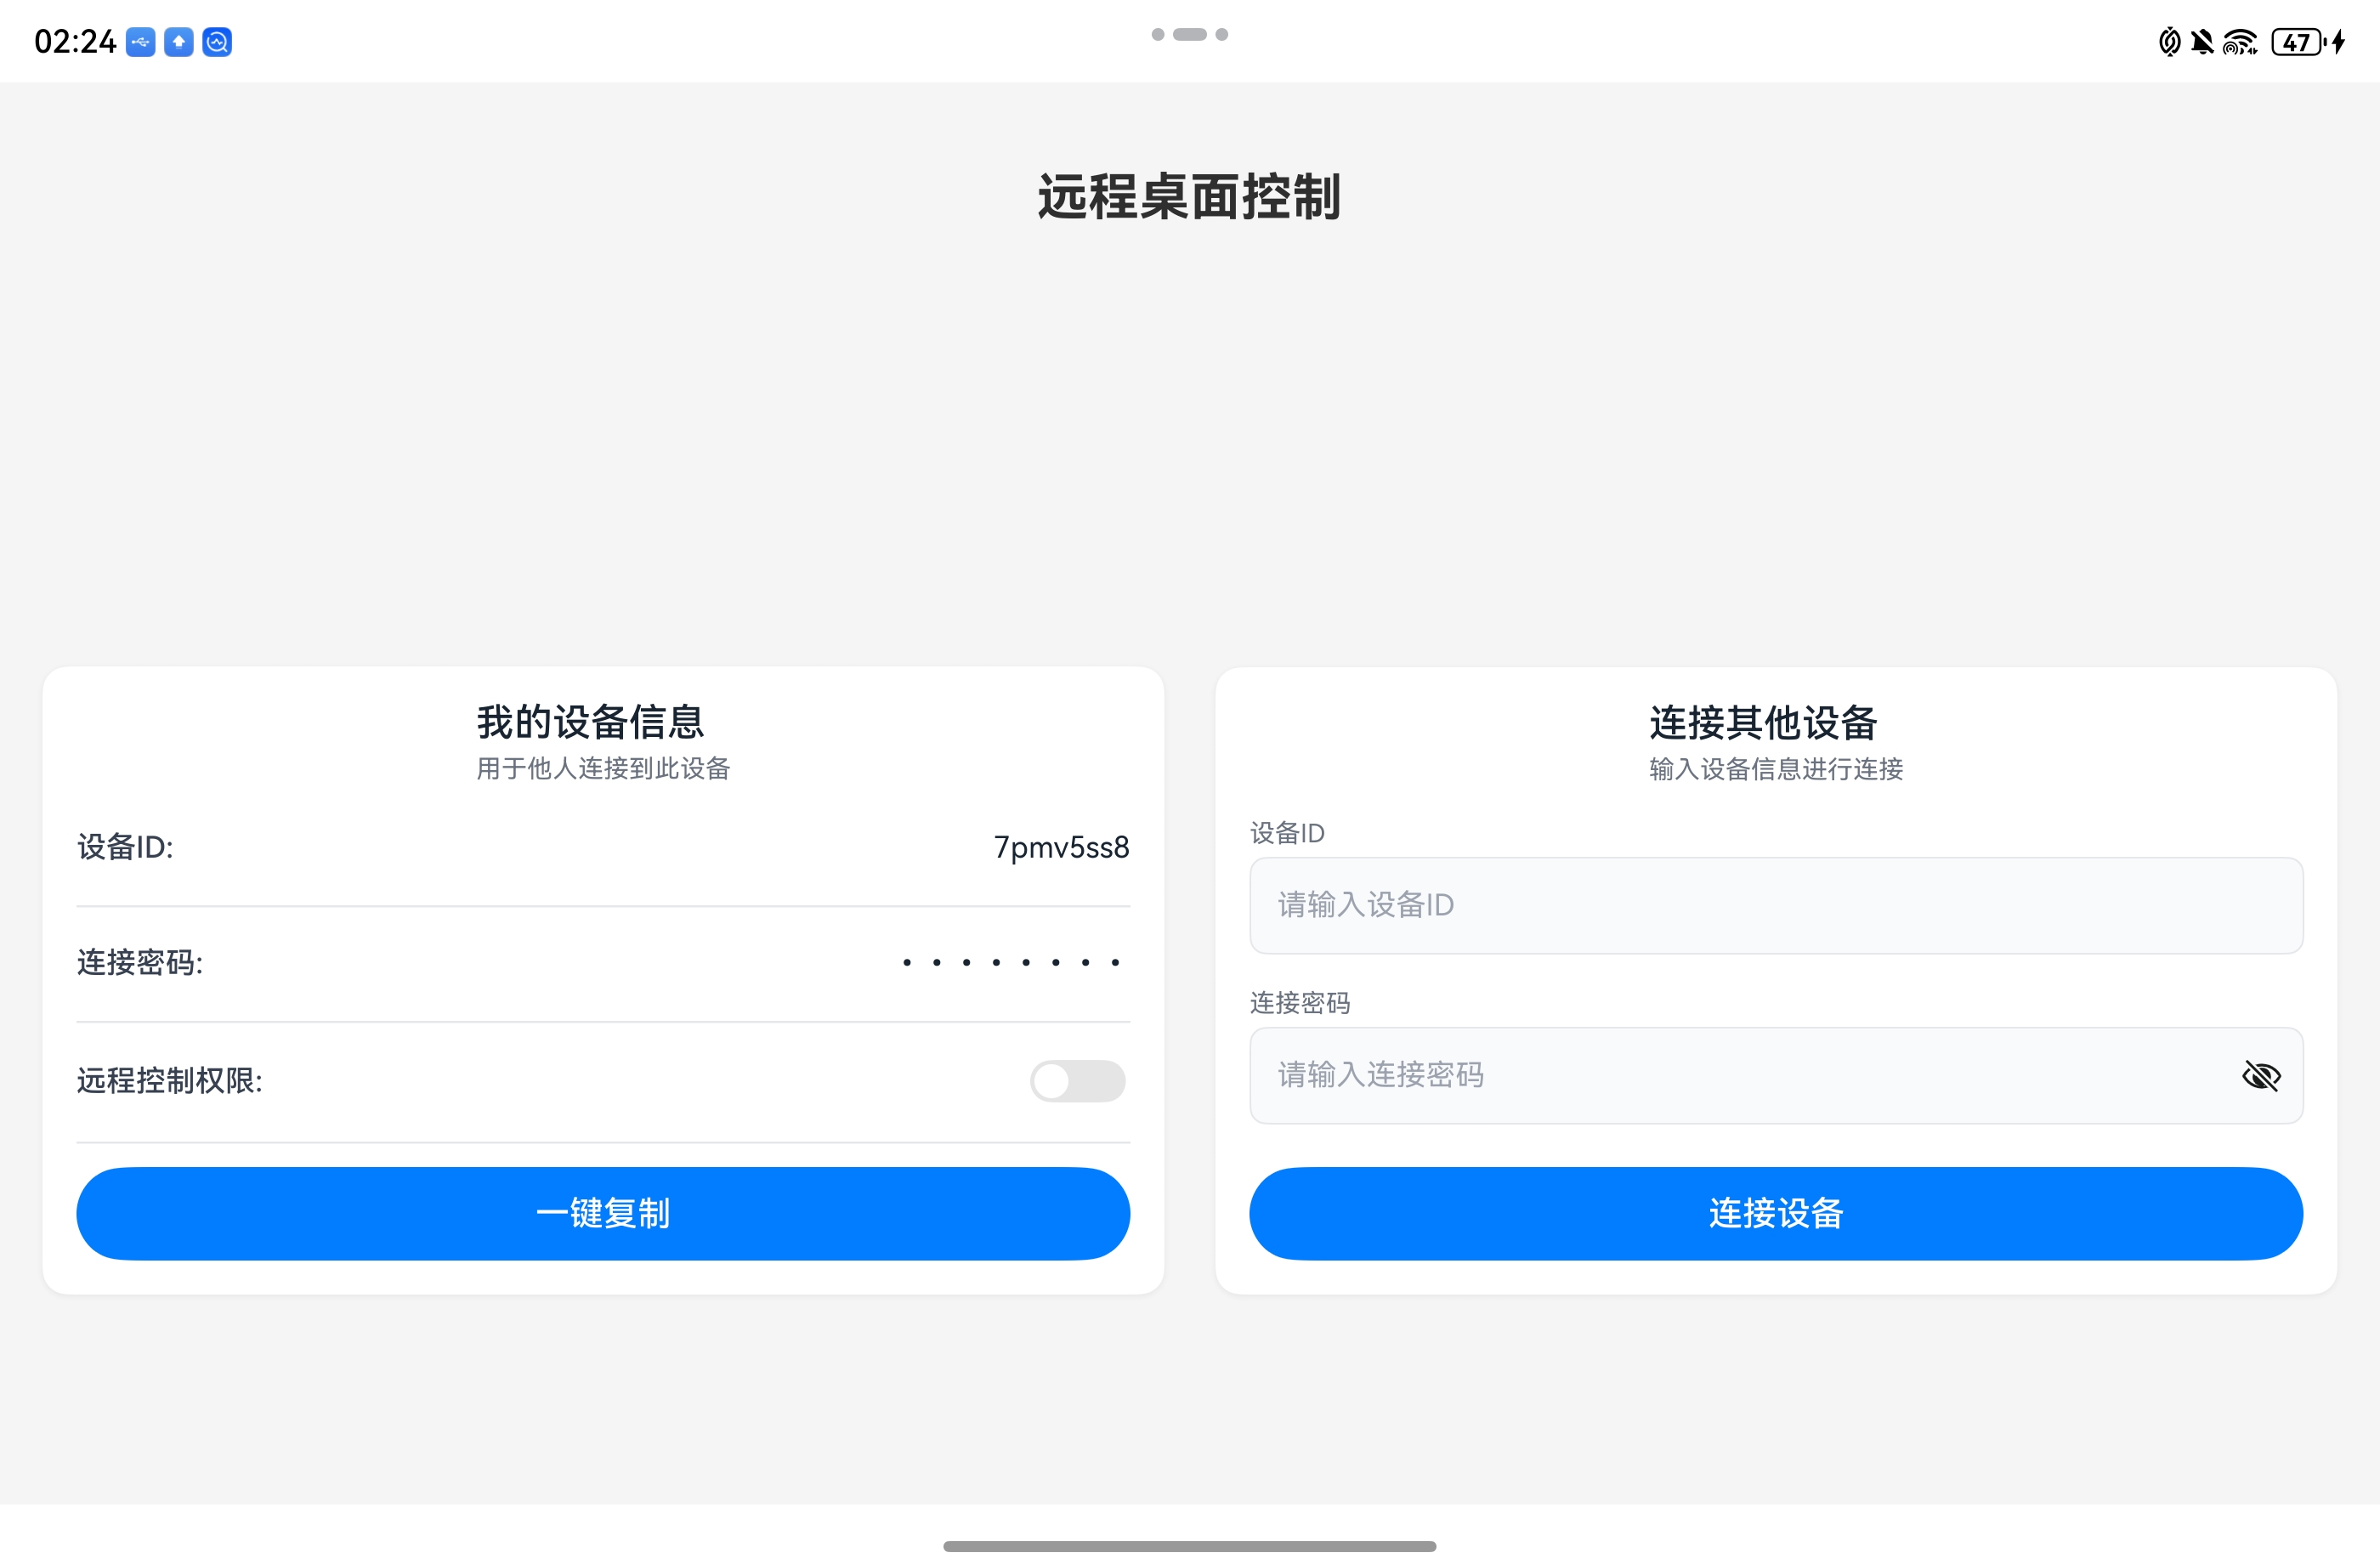
\includegraphics[width=0.92\textwidth]{../reference/picture/进入界面图.jpg}
\caption{进入界面图}
\end{figure}

\begin{figure}[h]
\centering
\includegraphics[width=0.92\textwidth]{../reference/picture/屏幕捕获与增量更新算法图.png}
\caption{屏幕捕获与增量更新算法图}
\end{figure}

\begin{figure}[h]
\centering
\includegraphics[width=0.92\textwidth]{../reference/picture/异步处理与背压控制图.png}
\caption{异步处理与背压控制图}
\end{figure}

\begin{figure}[h]
\centering
\includegraphics[width=0.92\textwidth]{../reference/picture/RLE + ZSTD 压缩算法.png}
\caption{RLE + ZSTD 压缩算法}
\end{figure}

\section{第四章\quad 测试报告}
请在本章描述测试方案、测试过程与测试结果。

\section{第五章\quad 安装及使用}
请在本章描述安装步骤与使用说明。

\section{第六章\quad 项目总结}
请在本章总结项目成果与改进方向。

\section*{参考文献}
\addcontentsline{toc}{section}{参考文献}
请在此列出参考文献。

\end{document}
